\documentclass[a4paper,12pt]{article}
\usepackage[a4paper]{geometry}
\geometry{top=1.0in, bottom=1.0in, left=0.1in, right=0.1in}
	%\pagestyle{plain}
\setlength{\textwidth}{150mm}
\setlength{\oddsidemargin}{0.1cm}
\setlength{\evensidemargin}{0.1cm}
\setlength{\marginparsep}{0.1cm}
\setlength{\marginparwidth}{0.1cm}
\setlength{\marginparpush}{0.1cm}

\usepackage[italian]{babel}
\usepackage{graphicx}
\usepackage[intlimits]{amsmath}
\usepackage{amsfonts}
%  \usepackage[pdftex]{graphicx}
 %  \usepackage{epstopdf}
%\usepackage{amsmath}
\usepackage{listings}
%\usepackage[margin=0.5in]{geometry}  
\addtolength{\oddsidemargin}{-.4in}
\addtolength{\evensidemargin}{-.4in}

\usepackage{color}


\begin{document}
\begin{center}
 \huge \bfseries {Zcms}
\\[0.5cm]
\end{center}
\section{Introduction}
Zcms is a content managent system based almost completely on javascript. It is designed to be lightweight and fast and to use ajax for content loading. Furthermore, it is possible to use mysql, xml or both technologies to store content datas. Building a website with zcms should be as simple as writing a basic xml file.
\section{Workflow of Zcms}
The first thing zcms does is loading resources/xml/config.xml, which is the main configuration of the site. The main config usually (but not mandatory) loads the css styles, add the layout divs (see Structure section), and sets global variables, like default target or default animation. Thereafter, the main config loads other external files, which can add articles, comments, html, php code or load in turn other files. Every external file must be loaded with a tag parameter that tells zcms which part of the file is to be added. Moreover, a target or a default target previosuly set must be provided (see Files Anatomy - Entries for further informations).
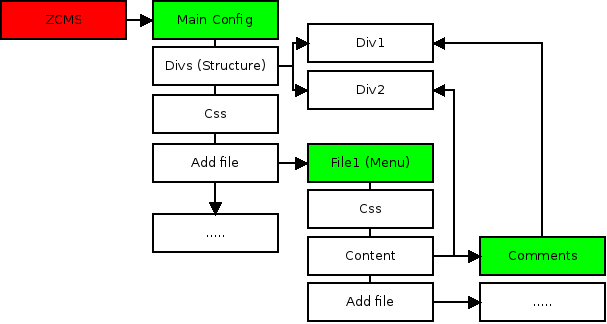
\includegraphics[scale=0.7]{Diagramma_zcms.png}
\section{Files Anatomy}
Every file is loaded with a tag parameter. Everything outside the tag is ignored and won't be loaded. For php files, the tag must be enclosed in at least one other element. For xml files, the tag can be the ancestor of the document.\\
There are 2 main sections: config and entries:
\begin{lstlisting}
 <tag>
<config>
...
</config>
<entry>
...
</entry>
<entry>
...
</entry>
\end{lstlisting}

\section{Structure}
Structure objects can be created using the following methods:
\subsection{js methods}
\begin{list}{-}{}
 \item Zcms.Structure.new\_div: this will create a simple div. Additional classes can be added.
\item Zcms.Structure.new\_tab: this will create an entry (\bfseries{TODO} \normalfont Rename to new\_entry?). An entry is a div with 2 or 3 subdivs: [title], content, comments. Each subdivs has 2 subdivs: \_text and \_text\_right
\end{list}
\subsection{xml methods}
\begin{list}{-}{}
  \item $<structure\_div>$: create a div and a subdiv \_content. It is created at the end of the current DOM, so it should be used only in the main config. It must be placed inside $<$config$>$ tag.
\item $<entry>$. Create a new tab. See the proper section for further informations.
\item 
\end{list}
\section{Config}
\bigskip
\bfseries{Note.}\normalfont If a php file is loaded through $<$load\_file$>$, the target tag must be a children of an element, otherwise it won't be loaded correctly. Xml files don't have this limitation.\\
\section{entry}
\subsection{tab}
\subsection{Comments}
Comments can be enabled or disabled in the single entry using the attribute \emph{comments}=\{'enabled','disabled'\}.\\
Comments must be located in resources/comments/\$entry\_id\$.xml.\\
A comment is an entry with \emph{type} attribute set to 'comment'. This ensures that zcms adds author of the comment and date to the entry tab.
Additionally, the entry div will have an \emph{id}='\$entry\_id\$\_comments' and \emph{class}='comments'.\\[0.2cm]
\bfseries{TODO}.\normalfont ATM configs inside entries are ignored (AFAIK). They can be introduced, allowing to unify tab and comments entries into one more dynamic paradigm.
\footnotesize
\lstset{language=XML}
\begin{lstlisting}
 <comments_$entry_id$ id="$entry_id$" target="#$entry_id$_comments_text" animation="enabled">
	<entry type="comment" id="1" author="m3l7" date="2011-09-07">
		<content>
			<span>Test comment</span>
		</content>
	</entry>
\end{lstlisting}


\end{document}